\chapter{条纹序、有限尺寸与超固态判据}
\label{ch:order-diagnostics}

\begin{learningobjectives}
完成本章后，读者应能：
\begin{enumerate}
  \item 用对称性不变的结构因子和有限尺寸标度诊断条纹长程序；
  \item 区分密度调制、相分离、显式钉扎与自发平移对称破缺；
  \item 为超固态结论同时检验密度序和超流响应；
  \item 对一维、有限温、非平衡和 TWA 晚时结果使用与证据相称的结论措辞。
\end{enumerate}
\end{learningobjectives}

\section{“有条纹”还不是超固态}

超固态的核心是两类性质共存\cite{Boninsegni2012}：
\begin{enumerate}
  \item 与平移对称破缺相关的晶体或密度波有序；
  \item 与全局 $U(1)$ 相位刚度相关的超流响应。
\end{enumerate}
一张单轨迹密度图出现周期起伏，只满足了最弱的候选信号。相分离后的畴壁、动力学不稳定的最快增长模、外势直接压出的密度波和有限采样噪声都能产生类似图样。反过来，对称性未显式破缺的有限系统中，系综平均密度可以完全均匀，而密度关联仍含有长程序。

因此本章不从“对比度是否非零”直接裁决超固态，而建立一组顺序明确的检验。

\section{条纹序参量与结构因子}

对长度 $L$ 的双分量 TWA 场，先定义正规排序总密度的单轨迹 Wigner 符号及其 Fourier 分量
\begin{equation}
  \begin{aligned}
  n_W^{(s)}(x)&=\sum_{\sigma=L,R}
  \left(|\psi_\sigma^{(s)}(x)|^2-\frac12\delta_{\mathcal C}(x,x)\right),\\
  M_Q^{(s)}&=\int_0^L\dd x\,\ee^{-\ii Qx}n_W^{(s)}(x),
  &N_W^{(s)}&=M_0^{(s)}.
  \end{aligned}
  \label{eq:trajectory-stripe-fourier-symbol}
\end{equation}
上标 $s$ 只是抽样轨迹编号，不代表一次物理单次测量；特别是低占据时，$N_W^{(s)}$ 可以有很大噪声，局部 $n_W^{(s)}$ 甚至可以为负。因此不应默认先形成随机比值 $M_Q^{(s)}/N_W^{(s)}$ 再平均。令 $\bar N=\ensavg{N_W}$，推荐使用比值--系综估计器
\begin{equation}
  \bar m_Q=\frac{\ensavg{M_Q}}{\bar N},
  \qquad
  \mathcal M_Q^2=
  \frac{\ensavg{|M_Q|^2}-C_Q^{(W)}}{\bar N^2}.
  \label{eq:ensemble-stripe-estimators}
\end{equation}
这里 $N_W^{(s)}=(\hat N)_W$ 已含每模半量子扣除；未扣除的原始模方和统一
记作 $\mathcal N_{\mathrm{sym}}^{(s)}$，两者不得互换。
第一项保留条纹平移相位，第二项是对称性不变的强度。若物理总粒子数在每个样本中被严格固定为同一个 $N$，才可等价地用固定分母 $M_Q^{(s)}/N$。

$C_Q^{(W)}$ 是\emph{双线性乘积}的 Weyl 接触修正，不能因 $Q\neq0$ 就遗漏。若 $M_Q$ 在保留的单粒子基中对应矩阵 $A_Q$，并且所选离散表示满足 $[A_Q,A_{-Q}]=0$，则
\begin{equation}
  C_Q^{(W)}=\frac14\Tr_{\mathcal C,\sigma}(A_QA_{-Q}).
  \label{eq:stripe-product-weyl-contact}
\end{equation}
在两个分量、$N_x$ 点的正交 collocation 格点且 $A_Q$ 只是格点相位时，$C_Q^{(W)}=N_x/2$。若先做谱投影再乘密度相位，截止边界可能使 $A_Q$ 与 $A_{-Q}$ 不对易；此时应直接计算该有限基中的完整星积，不能只套用式\eqref{eq:stripe-product-weyl-contact}的常数项。这个修正对宏观 Bragg 峰不改变热力学指数，却会污染低占据、小系统和无序基线。

无外场时，不同轨迹可以选择不同条纹原点，使
\begin{equation}
  \bar m_Q=0,
  \qquad
  \mathcal M_Q^2>0.
  \label{eq:symmetry-restored-stripe-ensemble}
\end{equation}
所以只看平均密度会漏检对称性恢复系综中的关联序。与第13章结构因子相连，在忽略不影响标度的规范差异时，Bragg 峰满足
\begin{equation}
  S_{\rm tot}(Q)=\frac{\ensavg{|M_Q|^2}-C_Q^{(W)}}{\bar N}
  =\bar N\mathcal M_Q^2,
  \qquad
  S_{\rm conn}(Q)=S_{\rm tot}(Q)-\bar N|\bar m_Q|^2.
  \label{eq:bragg-order-scaling}
\end{equation}
$S_{\rm tot}$ 保留显式钉扎或有限对称破缺场的弹性峰，$S_{\rm conn}$ 则扣掉平均密度调制。报告时必须说明采用哪一个。

固定密度取 $L,N\to\infty$ 时，三类标度可作初步区分：
\begin{center}
\begin{tabularx}{\textwidth}{p{0.25\textwidth}XX}
\toprule
密度关联 & $\mathcal M_Q^2$ & $S_{\rm tot}(Q)$ \\
\midrule
真正长程序 & 趋于非零常数 & 与 $N$ 成正比 \\
准长程序，$0<\eta<1$ & 约为 $L^{-\eta}$ & 约为 $L^{1-\eta}$ \\
有限关联长度 & 约为 $L^{-1}$ & 趋于常数量级 \\
\bottomrule
\end{tabularx}
\end{center}
这里假定振荡关联包络 $C_Q(r)\sim r^{-\eta}$。$\eta=0$ 对应真正长程序；$0<\eta<1$ 时积分给出上表幂律；$\eta=1$ 可出现对数修正；$\eta>1$ 时 $S(Q)$ 的领先项已为常数量级，仅靠该峰的幂指数不能再与有限关联长度区分。不能用单一尺寸区分这些情况。拟合时应比较“常数加有限尺寸修正”、幂律和有限相关长度模型，而不是预先选定最想看到的一个。

\section{波矢选择与峰值偏差}

目标 $Q$ 应优先由单粒子带极小值、Bogoliubov 软模或独立实验标定给出。若每条轨迹都在宽波数窗内寻找最大峰，再把最大值平均，即使无序噪声也会得到正偏差。可采用：
\begin{enumerate}
  \item 在独立训练数据上确定 $Q$ 和积分窗，在测试数据上估计强度；
  \item 对预注册的固定波数窗积分 Bragg 权重；
  \item 把完整寻峰算法应用到无序空模型，校准选择偏差；
  \item 在改变 $L$ 时保持物理波数窗，而不是保持固定 FFT 格点数。
\end{enumerate}

有限系统允许的离散波数可能不恰好包含理论 $Q$。应使用与边界相容的尺寸序列、扭曲边界或窗函数，并量化谱泄漏。把不同尺寸的最近 FFT 格点直接比较会把失配误判成序参量衰减。

\section{显式钉扎与自发破缺}

若哈密顿量含有 $h\cos(Qx)\hat n(x)$ 的外势，密度在有限 $h$ 下调制是显式响应。自发破缺的热力学定义要求按顺序取极限
\begin{equation}
  m_Q^{\rm SSB}=\lim_{h\to0^+}\lim_{L\to\infty}\qavg{m_Q}_{L,h}.
  \label{eq:ssb-order-of-limits}
\end{equation}
这里 $m_Q$ 表示正规排序密度算符除以物理 $N$，不是式\eqref{eq:trajectory-stripe-fourier-symbol}的单轨迹随机比值。有限尺寸、严格 $h=0$ 的精确本征态通常保持对称，故 $\qavg{m_Q}=0$ 并不排除热力学有序；有限 $h$ 下 $m_Q\neq0$ 也不证明自发有序。实际计算可结合零场 $\mathcal M_Q^2$ 标度、弱钉扎场响应和极限顺序。

Raman 光决定反冲波数，却未必等价于直接的密度晶格势。需要从实验室表象的完整哈密顿量判断条纹平移相位是自由集体坐标、只剩离散选择，还是已经被外场唯一钉扎。自旋轨道耦合凝聚体中“具有超固态性质的条纹相”已有实验实现\cite{Li2017}，但具体模型的对称性与诊断仍须逐项核对。

\section{超流性的独立检验}

密度序只是超固态的一半。对两个分量施加相同的边界扭转
\begin{equation}
  \psi_{L,R}(x+L)=\ee^{\ii\Theta}\psi_{L,R}(x),
  \label{eq:common-phase-twist-boundary}
\end{equation}
检验的是总质量 $U(1)$ 的相位刚度；相反扭转 $\Theta_L=-\Theta_R$ 检验的是自旋或相对相位刚度，二者不能互换。对一维平衡体系先定义无歧义的 helicity modulus
\begin{equation}
  \Upsilon=L\left.\frac{\partial^2F(\Theta)}{\partial\Theta^2}\right|_{\Theta=0},
  \label{eq:helicity-modulus-twist}
\end{equation}
其中零温时 $F$ 可换成基态能 $E$。只有在单一裸质量 $m$、普通 Galilean 归一化适用时，才进一步定义无量纲超流分数
\begin{equation}
  f_s=\frac{mL^2}{N\hbar^2}
  \left.\frac{\partial^2F(\Theta)}{\partial\Theta^2}\right|_{\Theta=0}.
  \label{eq:superfluid-fraction-twist}
\end{equation}
对 Galilean 不变、零温且完全超流的均匀体系，
$E(\Theta)-E(0)=N\hbar^2\Theta^2/(2mL^2)$，故 $f_s=1$。实际有限差分应成对计算
\begin{equation}
  F''(0)\simeq\frac{F(+\Theta)+F(-\Theta)-2F(0)}{\Theta^2},
  \label{eq:twist-central-difference}
\end{equation}
并扫描 $\Theta$ 以排除非线性响应。SOC 破坏普通 Galilean 不变性，响应可以是方向相关的张量，且用裸质量归一化出的量未必仍是 $[0,1]$ 内的“分数”；此时应优先报告共同规范扭转下的 $\Upsilon$ 或完整响应张量。规范表象中的扭转还要与 Raman 边界条件一致，不能只把 FFT 动量整体平移而保持激光相位约定不变。

其他互补指标包括：
\begin{enumerate}
  \item 一体密度矩阵最大本征值及 $g^{(1)}(r)$ 的长距离标度；
  \item 对弱矢势、缓慢移动边界或微小流速的线性电流响应；
  \item 平衡路径积分中的绕数涨落；
  \item 持久流稳定性与声学 Goldstone 响应。
\end{enumerate}
有限系统中宏观占据一个轨道不等于热力学超流刚度；反之，一维体系可以没有真正凝聚分数却保持有限相位刚度。应选择与维数、平衡/非平衡状态和可用方法相符的指标。

TWA 时间轨迹不能直接给出热力学自由能曲率。可在同一初态系综上施加成对的微小正负规范扭转或矢势，测量线性电流响应；若要声称平衡超流分数，还需证明所取状态和响应协议对应适当系综，并检查扰动幅度与等待时间极限。

\section{一维和有限温的限制}

在短程相互作用的一维体系中，连续对称性的涨落格外强。Hohenberg 定理排除热力学极限下有限温连续对称性的常规长程序\cite{Hohenberg1967}。零温低能区通常由 Luttinger 液体描述，相位和密度关联呈参数依赖的幂律\cite{Haldane1981,Cazalilla2004}；相应的密度波峰可以是代数奇点，而不是与体积成正比的真正 Bragg 峰。长程相互作用、晶格、显式钉扎或有限横向尺寸会改变结论，因此任何外推都必须重新检查理论前提。

因此，对准一维有限管中的“超固态”更稳健的表述可能是：在给定长度和时间窗内，观察到密度波关联与超流响应共存；其向热力学、长时间和严格一维极限的外推仍需标度。若只得到幂律密度序与幂律一体相干，可称为准长程序共存，而不宜无条件宣称严格长程超固态。

\section{淬火后条纹不是自动的平衡相}

淬火可以选择最快增长波矢并产生长寿命图样，但该图样可能是：
\begin{enumerate}
  \item 线性不稳定后的畴结构；
  \item 预热化平台中的准稳态关联；
  \item 守恒量约束下的非热稳态；
  \item 最终平衡有序相的早期成核；
  \item 截止相关经典场热化的暂态。
\end{enumerate}
要称为平衡超固态，需要在给定能量/温度和粒子数下独立建立平衡性。若只研究有限时间非平衡动力学，应使用“瞬态条纹序”“预热化密度波”或“超固态样共存”等更准确措辞。

相对相位在 $[0,2\pi)$ 上均匀也不能单独裁决。它可能意味着跨分量一阶相干消失；若 $M_Q^{(s)}$ 的相位跨轨迹随机而正规修正后的 $\mathcal M_Q^2$ 随尺寸保持，它也可能只是对称性恢复系综中条纹位置随机。反之，如果 $\mathcal M_Q^2\sim1/L$，才支持有限相关长度。必须把相位分布与幅度标度结合。

\section{一致的有限尺寸协议}

对 TWA 尺寸标度，建议保持以下物理量不变：
\begin{enumerate}
  \item 平均密度、相互作用常数、温度或单位粒子注入能；
  \item 物理格距或能量截止，而非格点总数；
  \item 边界条件、Raman 参数和目标 $Q$ 的物理窗口；
  \item 观测时间的物理定义，例如以声速穿越时间或碰撞时间归一；
  \item 每个尺寸下足以分辨 $S_{\rm tot}(Q)\sim N$ 与 $S_{\rm tot}(Q)\sim1$ 的轨迹数。
\end{enumerate}
固定密度和截止时，$N$ 与保留模式数 $M$ 都随 $L$ 增大，半量子总量也广延增长。这正是需要重复第9章截止稳定检查的原因。

推荐的判据矩阵如下：
\begin{center}
\begin{tabularx}{\textwidth}{p{0.22\textwidth}XX}
\toprule
主张 & 最低证据 & 关键反例排除 \\
\midrule
存在条纹关联 & $S_{\rm tot}(Q)$ 峰及实空间关联 & FFT 泄漏、寻峰偏差、外势 \\
长程密度序 & $S_{\rm tot}(Q)\propto N$ 或 $\mathcal M_Q^2\to c>0$ & 有限相关长度、畴平均 \\
存在超流性 & 扭转曲率或线性流响应 & 仅有凝聚峰、有限时间惯性 \\
超固态共存 & 同一状态中前两类证据同时成立 & 不同时间窗或不同参数拼接 \\
平衡自发破缺 & 尺寸、钉扎场和长时间极限 & 显式驱动、预热化暂态 \\
\bottomrule
\end{tabularx}
\end{center}

\section{实际随机相位标度基准}

配套程序生成两个明确的统计玩具模型，而不冒充完整凝聚体动力学：其一是整条系统具有随机全局条纹相位的有序系综，其二是固定相关长度的独立相位畴系综。所有密度场均由程序实际生成，结果见\cref{fig:stripe-scaling-toy}。
\begin{figure}[htbp]
  \centering
  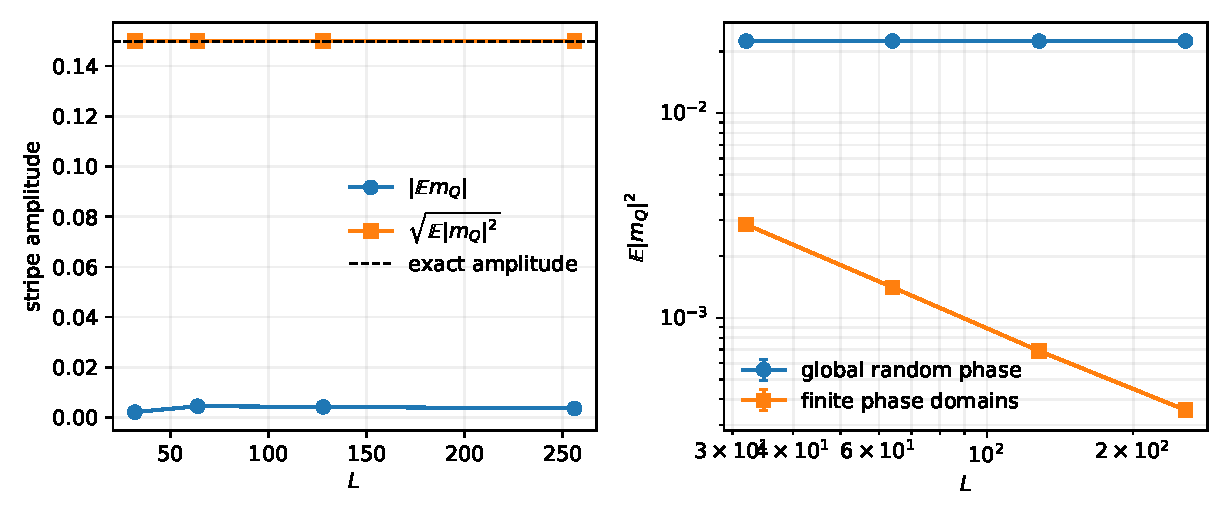
\includegraphics[width=0.78\textwidth]{figures/ch17/stripe_scaling_toy.pdf}
  \caption[条纹序有限尺寸标度的统计玩具模型]{条纹序有限尺寸标度的统计玩具模型。对 $L=32,64,128,256$，每个长度独立生成 $2000$ 条密度轨迹；右图误差棒为 $\pm1$ 标准误。随机全局相位系综的 $\mathcal M_Q^2$ 斜率在数值精度内为零，固定长度相位畴系综的对数斜率为 $-1.007\pm0.011$。该图演示“均值为零不等于无序”和有限尺寸判据，不是相互作用量子场的动力学证据。}
  \label{fig:stripe-scaling-toy}
\end{figure}
前者满足 $|\bar m_Q|\simeq0$ 但
$\mathcal M_Q^2$ 趋于常数；后者随 $L^{-1}$ 衰减。这个高占据经典玩具模型的程序变量沿用旧名 \texttt{m\_Q}，没有加入式\eqref{eq:stripe-product-weyl-contact}的量子接触项；将其迁移到 TWA 数据时必须加入该项。数据和拟合斜率保存在
\path{data/ch17/stripe_scaling_toy_metrics.json}。该基准只验证分析管线，不是本书对具体 Raman 参数下超固态的数值宣判。

\begin{chaptercheck}
只有当同一组参数和同一状态同时通过密度序标度、超流响应、显式钉扎排除、截止/步长/轨迹收敛和 TWA 有效时间检查，才把结论提升为“受 TWA 支持的超固态候选”。若还缺独立量子方法或平衡性证据，应把这些限制写进结论句本身。
\end{chaptercheck}

\section*{本章小结}

随机条纹相位会令平均密度均匀，却不抹去对称性不变的 Bragg 关联；真正长程序必须由 $S_{\rm tot}(Q)$ 或 $\mathcal M_Q^2$ 的尺寸标度识别。超固态还要求同一状态具有独立的共同 $U(1)$ 相位刚度。显式钉扎、一维涨落、非平衡暂态和 TWA 晚时截止效应都会降低可作结论的强度。相位均匀、条纹对比度下降或单尺寸 Bragg 峰都不能单独完成“自发对称破缺”的裁决。

\begin{exercises}
  \item 考虑随机全局相位的密度
  \[
    n(x)=n_0[1+A\cos(Qx+\theta)].
  \]
  计算 $\bar m_Q$ 与 $\mathcal M_Q^2$；在经典连续密度模型中取 $C_Q^{(W)}=0$。
  \item 设系统由 $L/\xi$ 个独立相位畴组成，推导 $\mathcal M_Q^2\propto\xi/L$。
  \item 从两个分量、$N_x$ 个格点模式的 Weyl 星积推导 $C_Q^{(W)}=N_x/2$，并估计遗漏该项对低占据 $S_{\rm tot}(Q)$ 的偏差。
  \item 验证式\eqref{eq:superfluid-fraction-twist}对均匀完全超流给出 $f_s=1$。
  \item 对 $C_Q(r)\sim\cos(Qr)r^{-\eta}$ 分别推导 $0<\eta<1$、$\eta=1$ 和 $\eta>1$ 时的有限尺寸标度。
  \item 设计尺寸与弱钉扎场的二维外推，以实现式\eqref{eq:ssb-order-of-limits}。
  \item 为“淬火后形成平衡超固态”列出一条可能否定该命题的最小数值结果。
\end{exercises}
